\section{Natural Clouds}

\subsection{Formation}
Clouds, as seen in nature, consist of a visible body of tiny water droplets and frozen crystals. 
In their natural occurrence, clouds are mostly generated from a nearby source of moisture, usually in the form of water vapor. 
This composition of particles creates the pleasant look of a white-grayish "fluffy" mass, floating in the sky.
\\
Due to certain factors like altitude or water source, different types of cloudscapes can be formed. They vary in shape, \gls{convection}, density and more.
That makes different cloud types highly unique in terms of appearance.
\\
For now, those factors are regarded as nature's randomness. However, an approximation of randomness will be covered in \sectionref{section:noise-generation}.


\subsection{Types of Clouds}
\label{section:cloud-types}
Cloudscapes are given a genus and classified in multiple groups, mainly differing in altitude, meaning the distance from the earth's surface to the cloud formation.
The following four cloud genera stand out due to their distinctiveness. A realistic simulation of a cloud system would consist of a combination of these types, which is why they are displayed here.
\begin{figure}[ht]
    \centering
        \begin{minipage}{0.47\linewidth}
            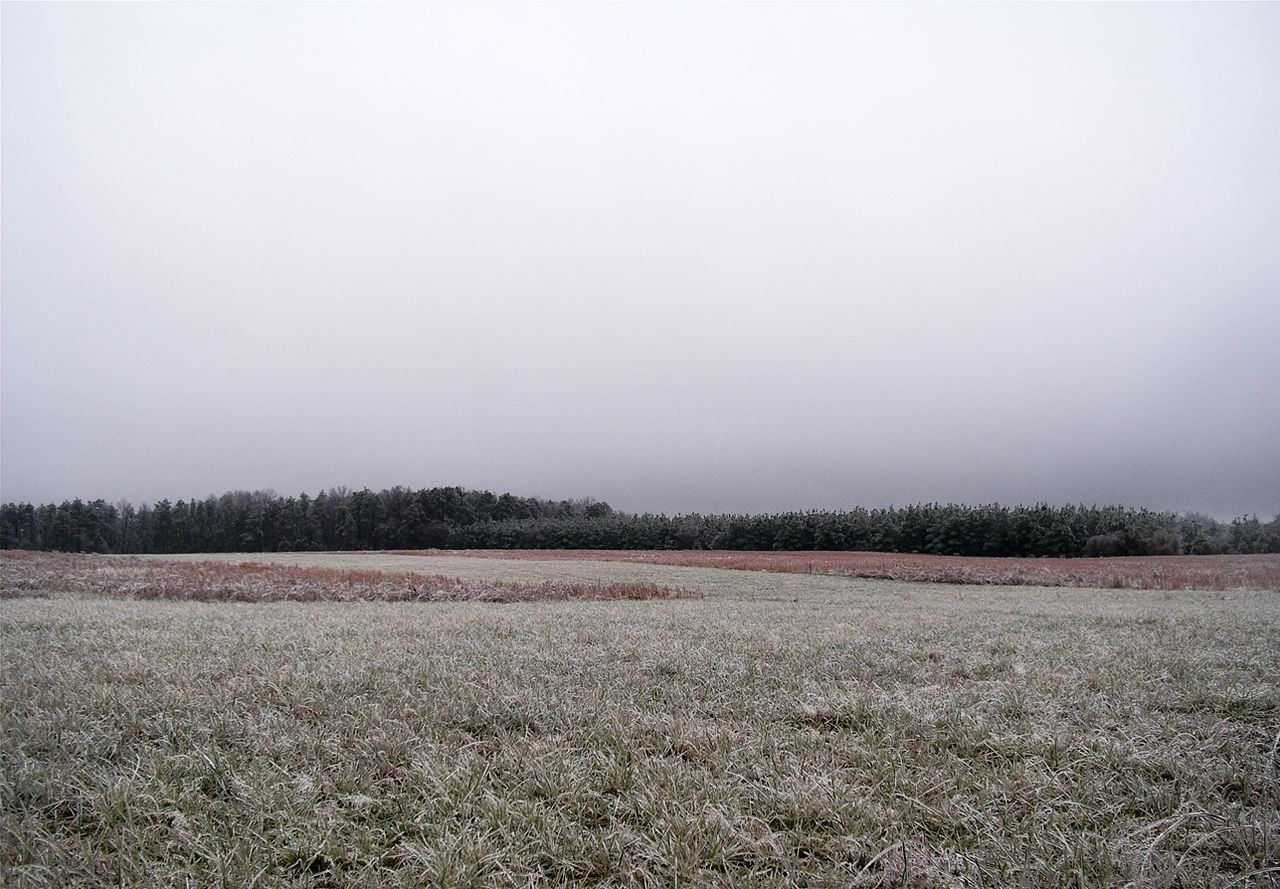
\includegraphics[width=\linewidth]{cloudforms-stratus}
            \captionof{figure}{Photographic reference of stratus clouds \protect\cite{img:cloudforms:stratus}.}
            \label{img:photo:cloudforms-stratus}        
        \end{minipage}        
    \hfill
        \begin{minipage}{0.47\linewidth}
            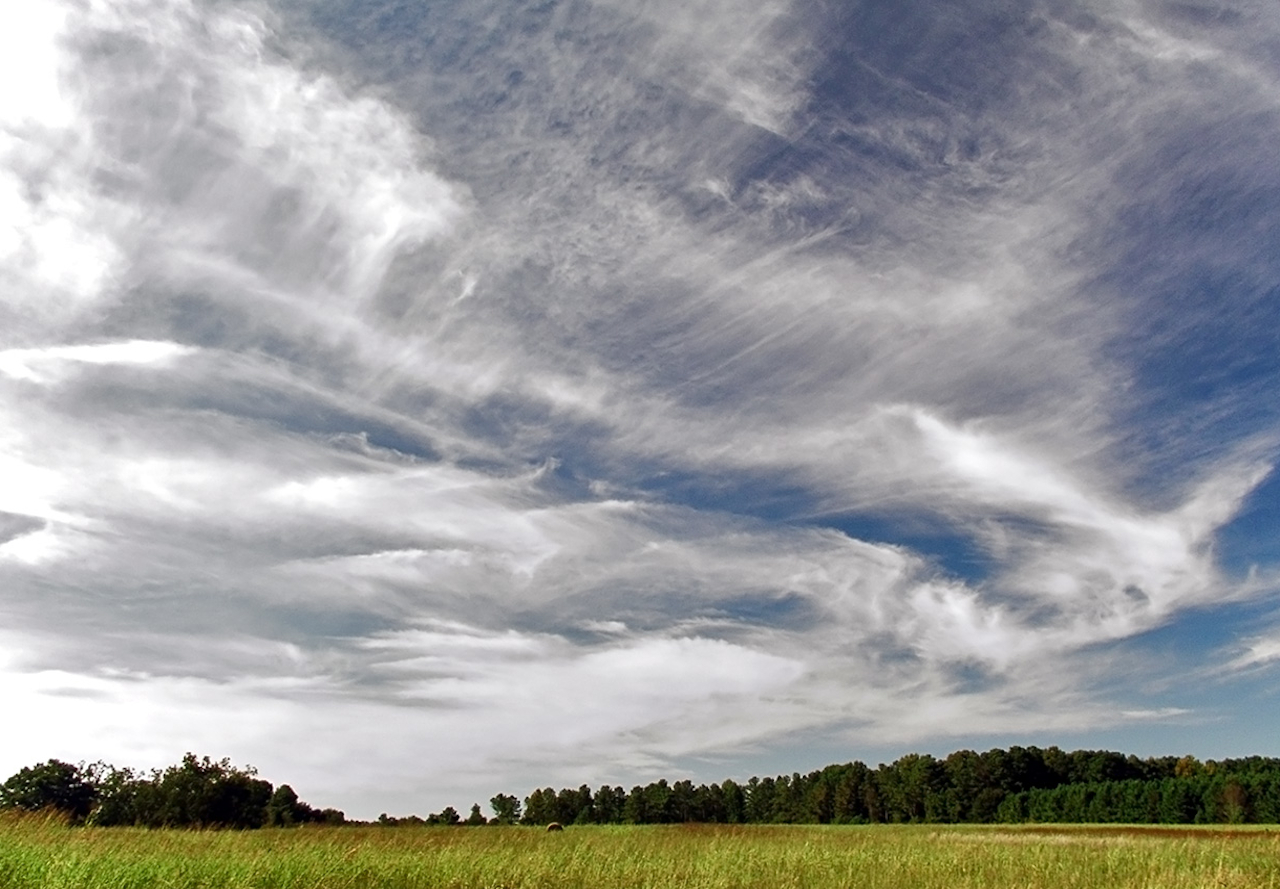
\includegraphics[width=\linewidth]{cloudforms-cirrus}
            \captionof{figure}{Photographic reference of cirrus clouds \protect\cite{img:cloudforms:cirrus}.}
            \label{img:photo:cloudforms-cirrus}        
        \end{minipage}
\end{figure}

\begin{figure}[ht]
    \centering
        \begin{minipage}{0.47\linewidth}
            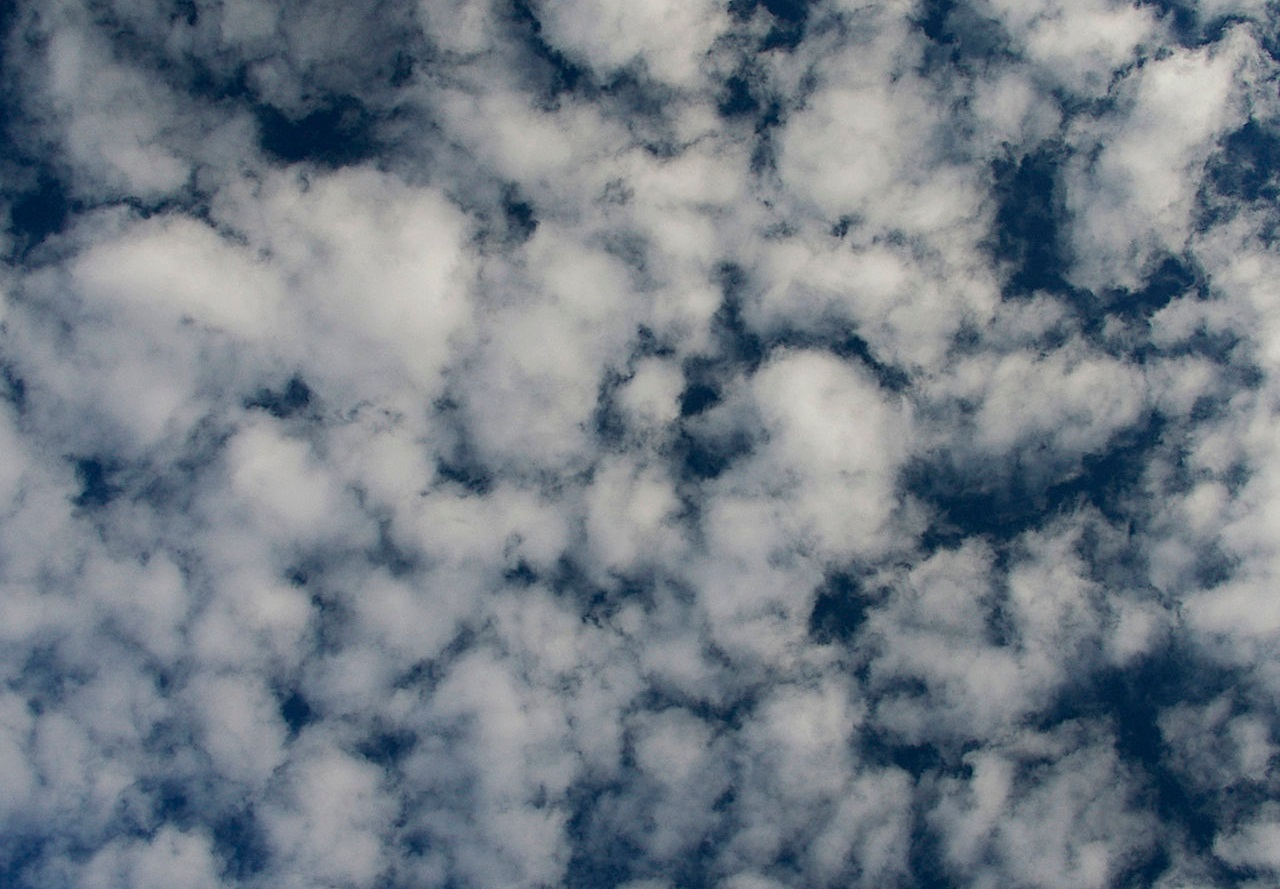
\includegraphics[width=\linewidth]{cloudforms-altocumulus}
            \captionof{figure}{Photographic reference of an altocumulus cloud formation \protect\cite{img:cloudforms:altocumulus}.}
            \label{img:photo:cloudforms-altocumulus}        
        \end{minipage}        
    \hfill
        \begin{minipage}{0.47\linewidth}
            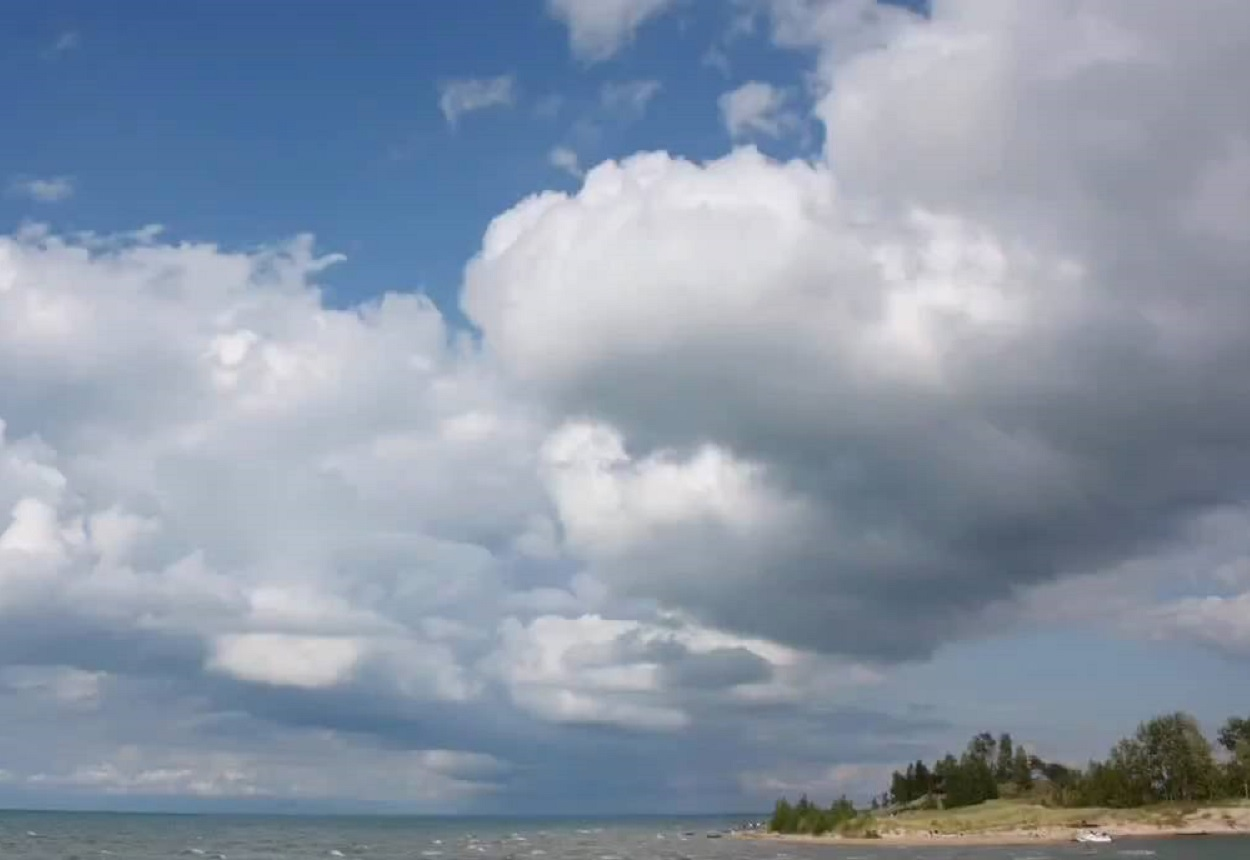
\includegraphics[width=\linewidth]{cloudforms-stratocumulus}
            \captionof{figure}{Photographic reference of stratocumulus cloudscape \protect\cite{img:cloudforms:stratocumulus}.}
            \label{img:photo:cloudforms-stratocumulus}        
        \end{minipage}
\end{figure}